\documentclass[../PianoDiProgetto_v3.0.0.tex]{subfiles}
\begin{document}

\section{Preventivo}
	\subsection{Stima}
		\subsubsection{Primo Periodo}
			\paragraph{Suddivisione del lavoro}
			Ogni componente del gruppo \kpanic\ rivestirà i seguenti ruoli:
			\begin{table}[h]
				%\centering
				\begin{tabularx}{\textwidth}{l * {6}{C} c}
				\toprule
				\textbf{Nominativo} & \textbf{Rp} & \textbf{Am} & \textbf{Pt} & \textbf{An} & \textbf{Pm} & \textbf{Ve} & \textbf{Ore totali} \\
				\midrule
				Berto Filippo &	0 & 13 & 0 & 12 & 0 & 5 & 30 \\
				%\midrule
				Fasolato Francesco & 9 & 9 & 0 & 0 & 0 & 12 & 30 \\
				%\midrule
				Favaro Daniele & 12 & 0 & 0 & 12 & 0 & 6 & 30 \\
				%\midrule
				Franceschini Marco & 0 & 9 & 0 & 12 & 0 & 9 & 30 \\
				%\midrule
				Macrì Antonino & 11 & 8 & 0 & 7 & 0 & 4 & 30 \\
				%\midrule
				Zanon Edoardo &	0 & 14 & 0 & 11 & 0 & 5 & 30 \\
				%\midrule
				Zecchin Giacomo & 0 & 11 & 0 & 14 & 0 & 5 & 30 \\
				\midrule			
				\textbf{Ore Totali Ruolo} & 32 & 64 & 0 & 68 & 0 & 46 & 210 \\
				\bottomrule
				\end{tabularx}
				\caption{Primo Periodo - Suddivisione delle ore di lavoro}		
			\end{table}

			Riassumendo la precedente tabella con un bar chart:	
			\begin{figure}[!h]
				\centering
				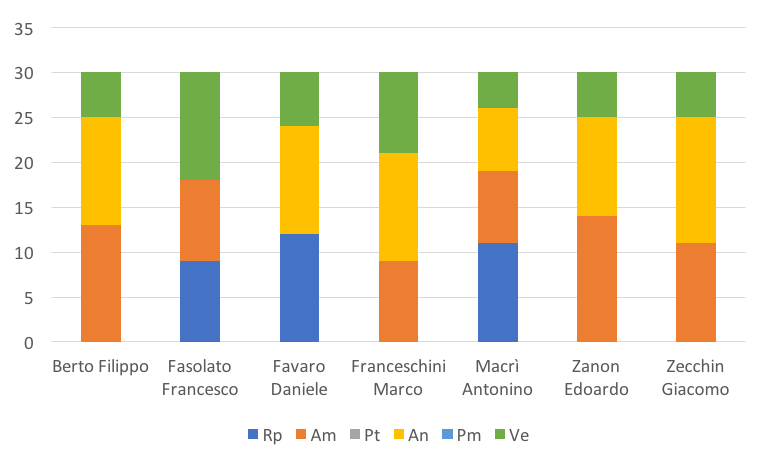
\includegraphics[width=\textwidth]{Preventivo/Immagini/fase1_oreRuoloPersona.png}
				\caption{Primo Periodo - Riassunto ore di lavoro per persona}
			\end{figure}	
			
			\newpage
			\paragraph{Prospetto economico}
			Il costo di ogni ruolo è indicato di seguito:
			\begin{table}[h]
				\centering
				\begin{tabular}{l * {2}{c}}
				\toprule
				\textbf{Ruolo} & \textbf{Ore} & \textbf{Costo (\euro{})} \\
				\midrule
				Responsabile & 32 & 960,00 \\
				%\midrule
				Amministratore & 64 & 1.280,00 \\
				%\midrule
				Progettista & 0 & 0,00 \\
				%\midrule
				Analista & 68 & 1.700,00 \\		
				%\midrule
				Programmatore & 0 & 0,00 \\		
				%\midrule
				Verificatore & 46 & 690,00 \\				
				\midrule		
				\textbf{Totale} & 210 & 4.630,00 \\
				\bottomrule	
				\end{tabular}
				\caption{Primo Periodo - Prospetto economico}		
			\end{table}
			
			Riassumendo la precedente tabella con due pie chart:	
			\begin{figure}[!h]
				\centering
				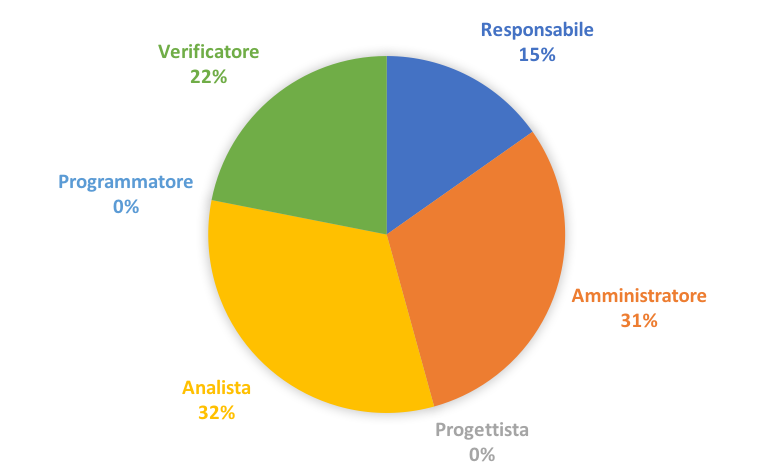
\includegraphics[width=\textwidth]{Preventivo/Immagini/fase1_oreRuolo.png}
				\caption{Primo Periodo - Riassunto ore di lavoro per ruolo}
			\end{figure}	
			\newpage
			\begin{figure}[!h]
				\centering
				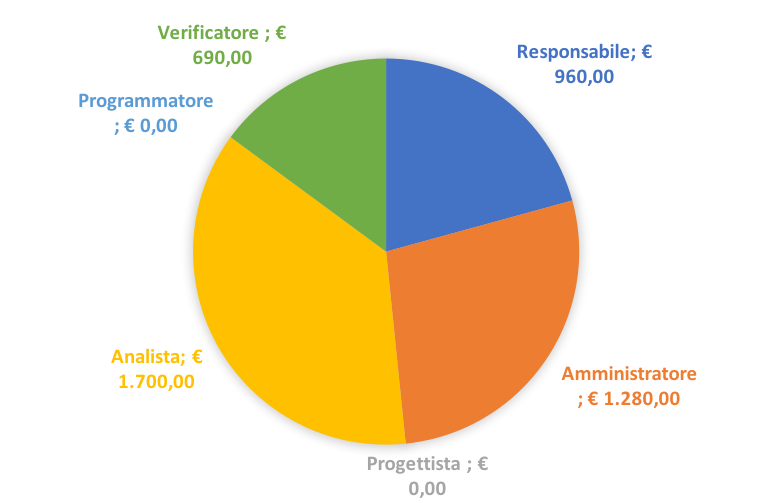
\includegraphics[width=\textwidth]{Preventivo/Immagini/fase1_costoRuolo.png}
				\caption{Primo Periodo - Riassunto costo per ruolo}
			\end{figure}	
			
		\newpage			
		\subsubsection{Secondo Periodo}
			\paragraph{Suddivisione del lavoro}
			Ogni componente del gruppo \kpanic\ rivestirà i seguenti ruoli:
			\begin{table}[h]
				%\centering
				\begin{tabularx}{\textwidth}{l * {6}{C} c}
				\toprule
				\textbf{Nominativo} & \textbf{Rp} & \textbf{Am} & \textbf{Pt} & \textbf{An} & \textbf{Pm} & \textbf{Ve} & \textbf{Ore totali} \\
				\midrule
				Berto Filippo &	0 & 0 & 0 & 4 & 0 & 5 & 9 \\
				%\midrule
				Fasolato Francesco & 0 & 5 & 0 & 4 & 0 & 0 & 9 \\
				%\midrule
				Favaro Daniele & 0 & 4 & 0 & 0 & 0 & 6 & 10 \\
				%\midrule
				Franceschini Marco & 0 & 0 & 0 & 3 & 0 & 6 & 9 \\
				%\midrule
				Macrì Antonino & 0 & 0 & 0 & 4 & 0 & 5 & 9 \\
				%\midrule
				Zanon Edoardo &	5 & 0 & 0 & 3 & 0 & 2 & 10 \\
				%\midrule
				Zecchin Giacomo & 4 & 0 & 0 & 0 & 0 & 6 & 10 \\
				\midrule			
				\textbf{Ore Totali Ruolo} & 9 & 9 & 0 & 18 & 0 & 30 & 66 \\
				\bottomrule
				\end{tabularx}
				\caption{Secondo Periodo - Suddivisione delle ore di lavoro}		
			\end{table}
			
			Riassumendo la precedente tabella con un bar chart:	
			\begin{figure}[!h]
				\centering
				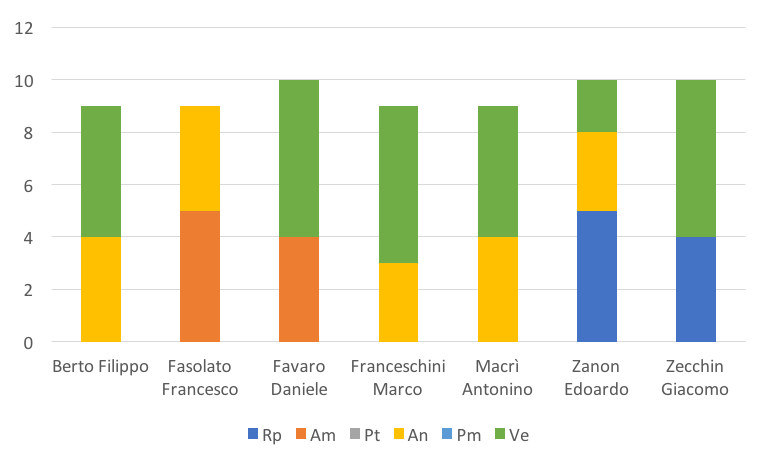
\includegraphics[width=\textwidth]{Preventivo/Immagini/fase2_oreRuoloPersona.png}
				\caption{Secondo Periodo - Riassunto ore di lavoro per persona}
			\end{figure}	
			
			\newpage
			\paragraph{Prospetto economico}
			Il costo di ogni ruolo è indicato di seguito:
			\begin{table}[h]
				\centering
				\begin{tabular}{l * {2}{c}}
				\toprule
				\textbf{Ruolo} & \textbf{Ore} & \textbf{Costo (\euro{})} \\
				\midrule
				Responsabile & 9 & 270,00 \\
				%\midrule
				Amministratore & 9 & 180,00 \\
				%\midrule
				Progettista & 0 & 0,00 \\
				%\midrule
				Analista & 18 & 450,00 \\		
				%\midrule
				Programmatore & 0 & 0,00 \\		
				%\midrule
				Verificatore & 30 & 450,00 \\				
				\midrule		
				\textbf{Totale} & 66 & 1.350,00 \\
				\bottomrule	
				\end{tabular}
				\caption{Secondo Periodo - Prospetto economico}		
			\end{table}
			
			Riassumendo la precedente tabella con due pie chart:	
			\begin{figure}[!h]
				\centering
				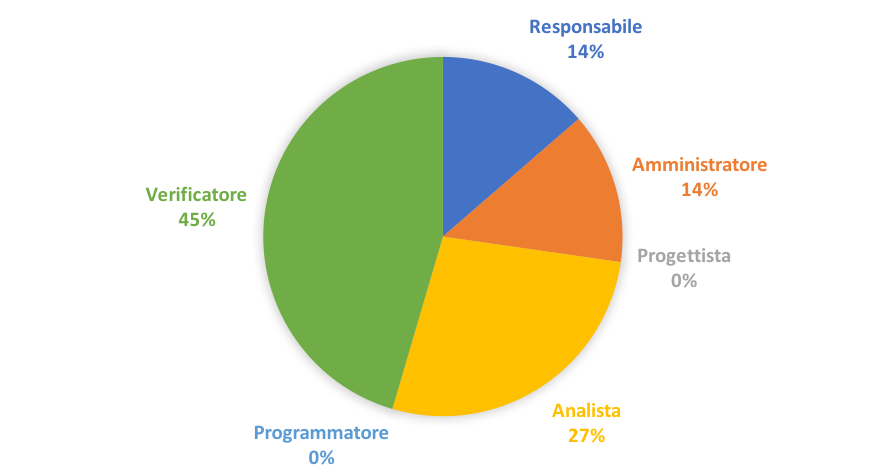
\includegraphics[width=\textwidth]{Preventivo/Immagini/fase2_oreRuolo.png}
				\caption{Secondo Periodo - Riassunto ore di lavoro per ruolo}
			\end{figure}	
			\newpage
			\begin{figure}[!h]
				\centering
				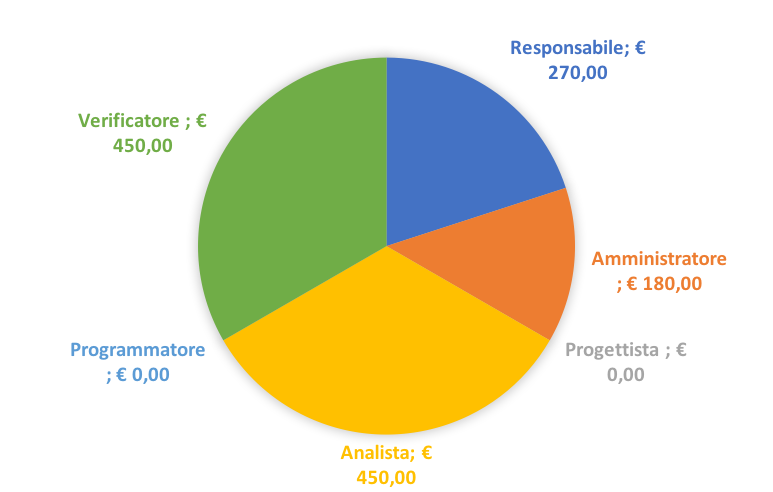
\includegraphics[width=\textwidth]{Preventivo/Immagini/fase2_costoRuolo.png}
				\caption{Secondo Periodo - Riassunto costo per ruolo}
			\end{figure}	
			
		\newpage
		\subsubsection{Terzo Periodo}
			\paragraph{Suddivisione del lavoro}
			Ogni componente del gruppo \kpanic\ rivestirà i seguenti ruoli:
			\begin{table}[h]
				%\centering
				\begin{tabularx}{\textwidth}{l * {6}{C} c}
				\toprule
				\textbf{Nominativo} & \textbf{Rp} & \textbf{Am} & \textbf{Pt} & \textbf{An} & \textbf{Pm} & \textbf{Ve} & \textbf{Ore totali} \\
				\midrule
				Berto Filippo &	0 & 0 & 18 & 7 & 0 & 0 & 25 \\
				%\midrule
				Fasolato Francesco & 0 & 0 & 17 & 0 & 0 & 7 & 24 \\
				%\midrule
				Favaro Daniele & 0 & 0 & 17 & 0 & 0 & 7 & 24 \\
				%\midrule
				Franceschini Marco & 17	& 0 & 0 & 0 & 0 & 7 & 24 \\
				%\midrule
				Macrì Antonino & 0 & 8 & 0 & 11 & 0 & 5 & 24 \\
				%\midrule
				Zanon Edoardo &	0 & 0 & 18 & 7 & 0 & 0 & 25 \\
				%\midrule
				Zecchin Giacomo & 0 & 8 & 0 & 11 & 0 & 5 & 24 \\
				\midrule			
				\textbf{Ore Totali Ruolo} & 17 & 16 & 70 & 36 & 0 & 31 & 170 \\
				\bottomrule
				\end{tabularx}
				\caption{Terzo Periodo - Suddivisione delle ore di lavoro}		
			\end{table}
			
			Riassumendo la precedente tabella con un bar chart:	
			\begin{figure}[!h]
				\centering
				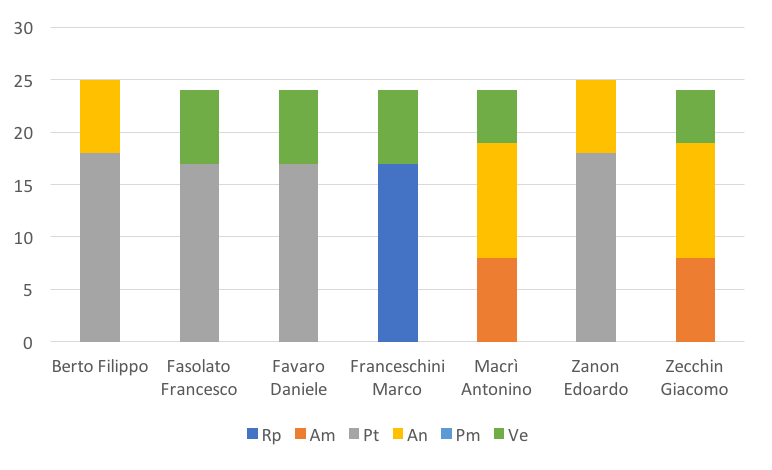
\includegraphics[width=\textwidth]{Preventivo/Immagini/fase3_oreRuoloPersona.png}
				\caption{Terzo Periodo - Riassunto ore di lavoro per persona}
			\end{figure}	
			
			\newpage
			\paragraph{Prospetto economico}
			Il costo di ogni ruolo è indicato di seguito:
			\begin{table}[h]
				\centering
				\begin{tabular}{l * {2}{c}}
				\toprule
				\textbf{Ruolo} & \textbf{Ore} & \textbf{Costo (\euro{})} \\
				\midrule
				Responsabile & 17 & 510,00 \\
				%\midrule
				Amministratore & 16 & 320,00 \\
				%\midrule
				Progettista & 70 & 1.540,00 \\
				%\midrule
				Analista & 36 & 900,00 \\		
				%\midrule
				Programmatore & 0 & 0,00 \\		
				%\midrule
				Verificatore & 31 & 465,00 \\				
				\midrule		
				\textbf{Totale} & 170 & 3.735,00 \\
				\bottomrule	
				\end{tabular}
				\caption{Terzo Periodo - Prospetto economico}		
			\end{table}
			
			Riassumendo la precedente tabella con due pie chart:	
			\begin{figure}[!h]
				\centering
				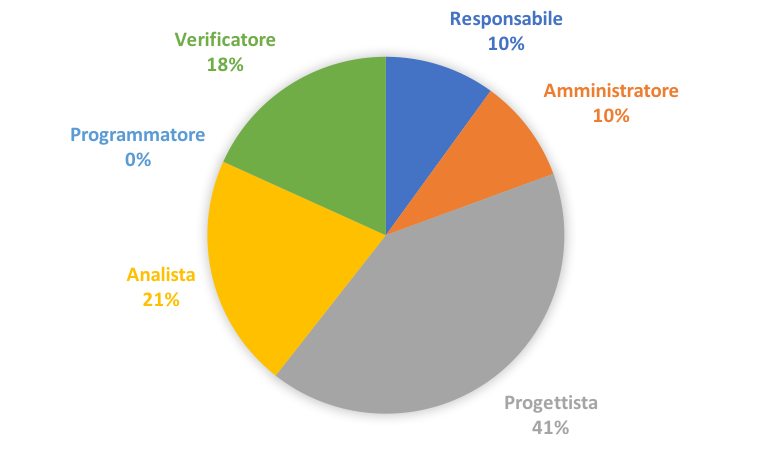
\includegraphics[width=\textwidth]{Preventivo/Immagini/fase3_oreRuolo.png}
				\caption{Terzo Periodo - Riassunto ore di lavoro per ruolo}
			\end{figure}
			\newpage
			\begin{figure}[!h]
				\centering
				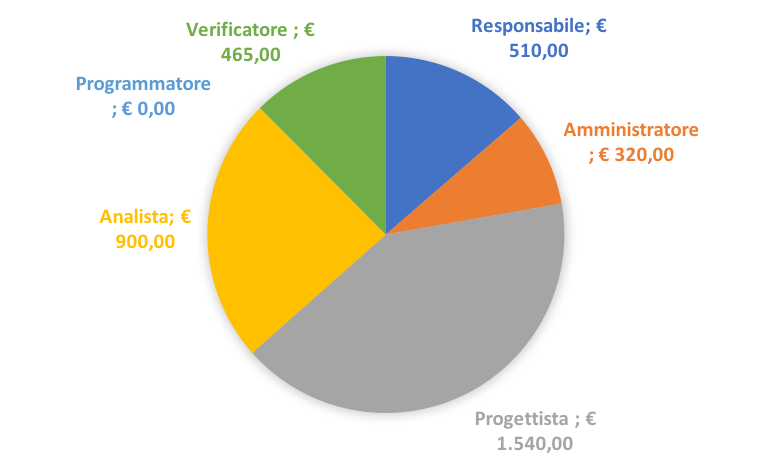
\includegraphics[width=\textwidth]{Preventivo/Immagini/fase3_costoRuolo.png}
				\caption{Terzo Periodo - Riassunto costo per ruolo}
			\end{figure}		

		\newpage
		\subsubsection{Quarto Periodo}
			\paragraph{Suddivisione del lavoro}
			Ogni componente del gruppo \kpanic\ rivestirà i seguenti ruoli:
			\begin{table}[h]
				%\centering
				\begin{tabularx}{\textwidth}{l * {6}{C} c}
				\toprule
				\textbf{Nominativo} & \textbf{Rp} & \textbf{Am} & \textbf{Pt} & \textbf{An} & \textbf{Pm} & \textbf{Ve} & \textbf{Ore totali} \\
				\midrule
				Berto Filippo &	13 & 0 & 0 & 0 & 15 & 0 & 28 \\
				%\midrule
				Fasolato Francesco & 0 & 5 & 0 & 5 & 6 & 14 & 30 \\
				%\midrule
				Favaro Daniele & 0 & 0 & 0 & 0 & 13 & 16 & 29 \\
				%\midrule
				Franceschini Marco & 0 & 0 & 9 & 0 & 20 & 0 & 29 \\
				%\midrule
				Macrì Antonino & 0 & 5 & 9 & 0 & 6 & 11 & 31 \\
				%\midrule
				Zanon Edoardo &	0 & 0 & 9 & 0 & 18 & 5 & 32 \\
				%\midrule
				Zecchin Giacomo & 0 & 0 & 9 & 0 & 18 & 5 & 32 \\
				\midrule			
				\textbf{Ore Totali Ruolo} & 13 & 10 & 36 & 5 & 96 & 51 & 211 \\
				\bottomrule
				\end{tabularx}
				\caption{Quarto Periodo - Suddivisione delle ore di lavoro}		
			\end{table}
			
			Riassumendo la precedente tabella con un bar chart:	
			\begin{figure}[!h]
				\centering
				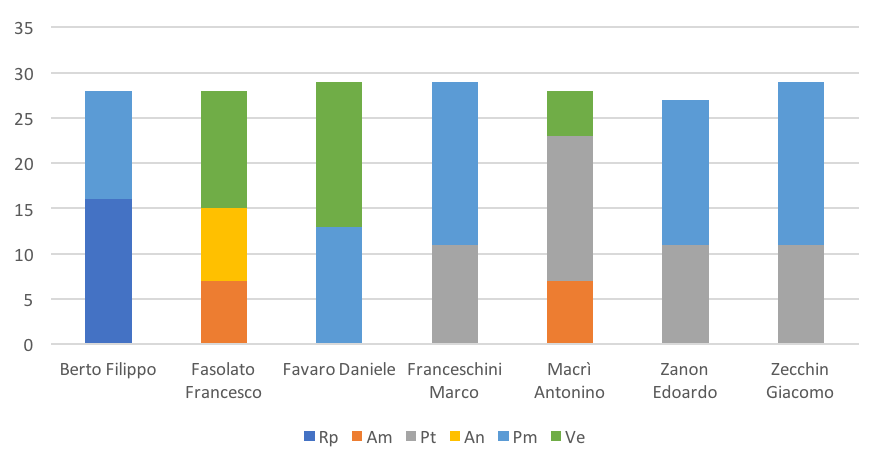
\includegraphics[width=\textwidth]{Preventivo/Immagini/fase4_oreRuoloPersona.png}
				\caption{Quarto Periodo - Riassunto ore di lavoro per persona}
			\end{figure}	
			
			\newpage
			\paragraph{Prospetto economico}
			Il costo di ogni ruolo è indicato di seguito:
			\begin{table}[h]
				\centering
				\begin{tabular}{l * {2}{c}}
				\toprule
				\textbf{Ruolo} & \textbf{Ore} & \textbf{Costo (\euro{})} \\
				\midrule
				Responsabile & 13 & 390,00 \\
				%\midrule
				Amministratore & 10 & 200,00 \\
				%\midrule
				Progettista & 36 & 792,00 \\
				%\midrule
				Analista & 5 & 125,00 \\		
				%\midrule
				Programmatore & 96 & 1.440,00 \\		
				%\midrule
				Verificatore & 51 & 765,00 \\				
				\midrule		
				\textbf{Totale} & 211 & 3.712,00 \\
				\bottomrule	
				\end{tabular}
				\caption{Quarto Periodo - Prospetto economico}		
			\end{table}
			
			Riassumendo la precedente tabella con due pie chart:	
			\begin{figure}[!h]
				\centering
				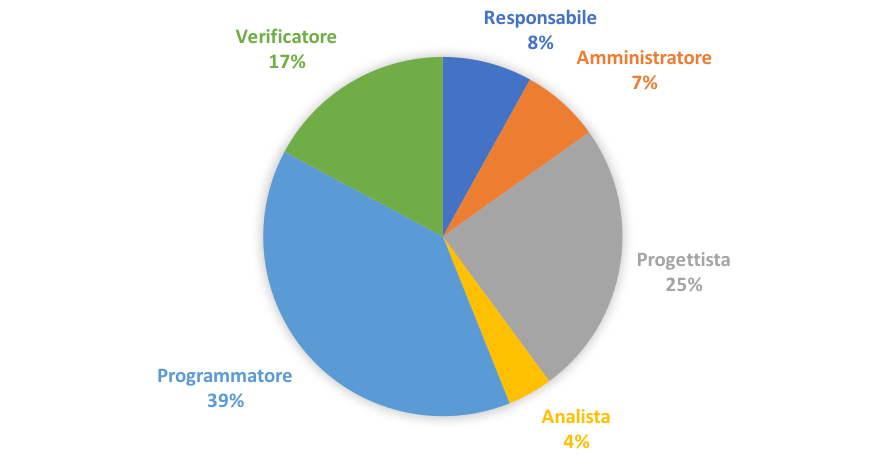
\includegraphics[width=\textwidth]{Preventivo/Immagini/fase4_oreRuolo.png}
				\caption{Quarto Periodo - Riassunto ore di lavoro per ruolo}
			\end{figure}	
			\newpage
			\begin{figure}[!h]
				\centering
				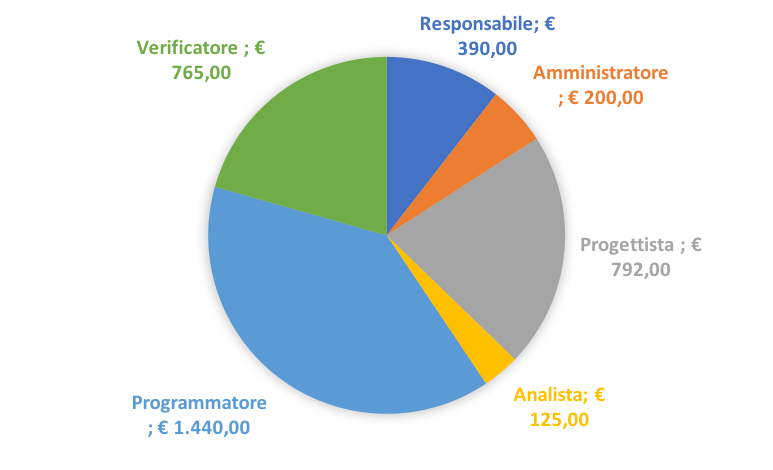
\includegraphics[width=\textwidth]{Preventivo/Immagini/fase4_costoRuolo.png}
				\caption{Quarto Periodo - Riassunto costo per ruolo}
			\end{figure}	
		
		\newpage
		\subsubsection{Quinto Periodo}
			\paragraph{Suddivisione del lavoro}
			Ogni componente del gruppo \kpanic\ rivestirà i seguenti ruoli:
			\begin{table}[h]
				%\centering
				\begin{tabularx}{\textwidth}{l * {6}{C} c}
				\toprule
				\textbf{Nominativo} & \textbf{Rp} & \textbf{Am} & \textbf{Pt} & \textbf{An} & \textbf{Pm} & \textbf{Ve} & \textbf{Ore totali} \\
				\midrule
				Berto Filippo &	0 & 0 & 0 & 5 & 5 & 7 & 17 \\
				%\midrule
				Fasolato Francesco & 0 & 0 & 5 & 3 & 0 & 7 & 15 \\
				%\midrule
				Favaro Daniele & 0 & 5 & 0 & 5 & 0 & 6 & 16 \\
				%\midrule
				Franceschini Marco & 0 & 0 & 0 & 0 & 10 & 7 & 17 \\
				%\midrule
				Macrì Antonino & 0 & 0 & 0 & 0 & 10 & 5 & 15 \\
				%\midrule
				Zanon Edoardo &	10 & 0 & 0 & 0 & 5 & 0 & 15 \\
				%\midrule
				Zecchin Giacomo & 0 & 0 & 4 & 0 & 3 & 7 & 14 \\
				\midrule		
				\textbf{Ore Totali Ruolo} & 10 & 5 & 9 & 13 & 33 & 39 & 109 \\
				\bottomrule
				\end{tabularx}
				\caption{Quinto Periodo - Suddivisione delle ore di lavoro}		
			\end{table}

			Riassumendo la precedente tabella con un bar chart:	
			\begin{figure}[!h]
				\centering
				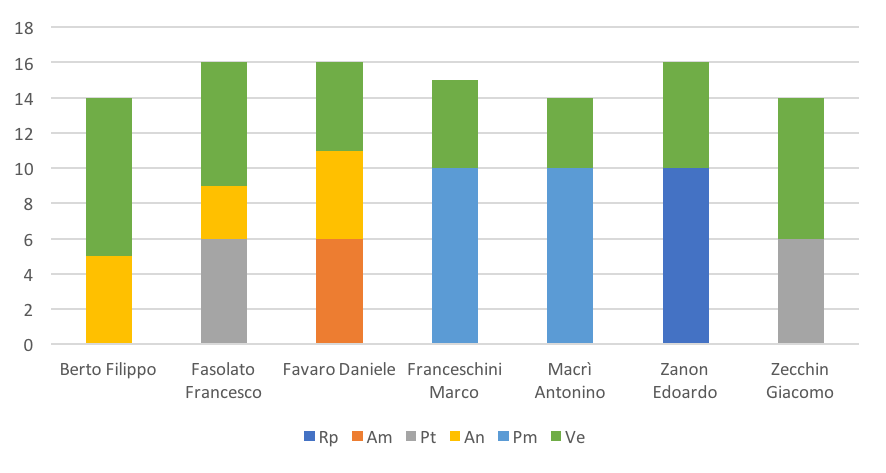
\includegraphics[width=\textwidth]{Preventivo/Immagini/fase5_oreRuoloPersona.png}
				\caption{Quinto Periodo - Riassunto ore di lavoro per persona}
			\end{figure}	
			
			\newpage
			\paragraph{Prospetto economico}
			Il costo di ogni ruolo è indicato di seguito:
			\begin{table}[h]
				\centering
				\begin{tabular}{l * {2}{c}}
				\toprule
				\textbf{Ruolo} & \textbf{Ore} & \textbf{Costo (\euro{})} \\
				\midrule
				Responsabile & 10 & 300,00 \\
				%\midrule
				Amministratore & 5 & 100,00 \\
				%\midrule
				Progettista & 9 & 198,00 \\
				%\midrule
				Analista & 13 & 325,00 \\		
				%\midrule
				Programmatore & 32 & 480,00 \\		
				%\midrule
				Verificatore & 38 & 570,00 \\				
				\midrule		
				\textbf{Totale} & 109 & 1.973,00 \\
				\bottomrule	
				\end{tabular}
				\caption{Quinto Periodo - Prospetto economico}		
			\end{table}
			
			Riassumendo la precedente tabella con due pie chart:	
			\begin{figure}[!h]
				\centering
				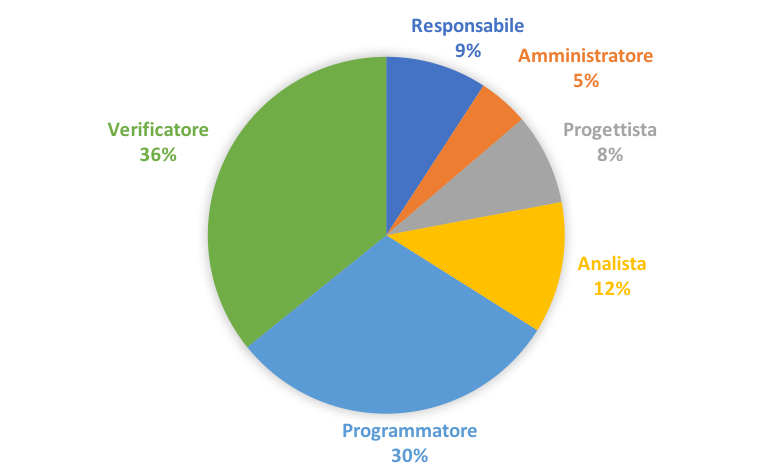
\includegraphics[width=\textwidth]{Preventivo/Immagini/fase5_oreRuolo.png}
				\caption{Quinto Periodo - Riassunto ore di lavoro per ruolo}
			\end{figure}
			\newpage	
			\begin{figure}[!h]
				\centering
				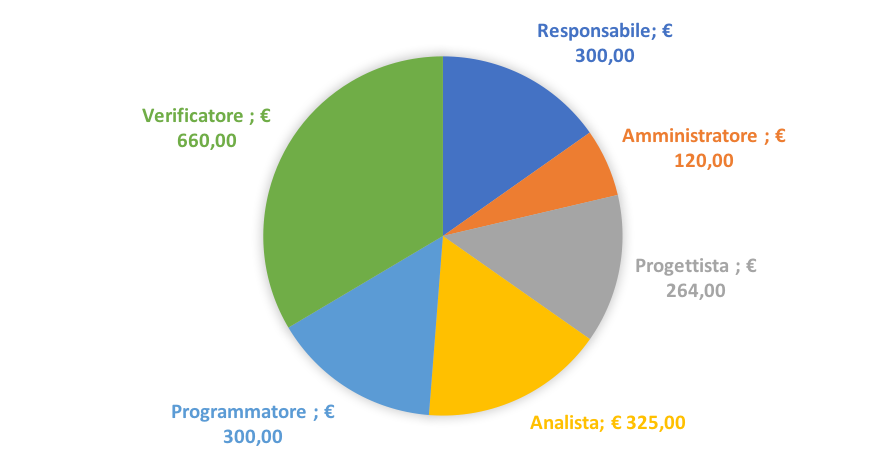
\includegraphics[width=\textwidth]{Preventivo/Immagini/fase5_costoRuolo.png}
				\caption{Quinto Periodo - Riassunto costo per ruolo}
			\end{figure}	
			
		\newpage
		\subsubsection{Sesto Periodo}
			\paragraph{Suddivisione del lavoro}
			Ogni componente del gruppo \kpanic\ rivestirà i seguenti ruoli:
			\begin{table}[h]
				%\centering
				\begin{tabularx}{\textwidth}{l * {6}{C} c}
				\toprule
				\textbf{Nominativo} & \textbf{Rp} & \textbf{Am} & \textbf{Pt} & \textbf{An} & \textbf{Pm} & \textbf{Ve} & \textbf{Ore totali} \\
				\midrule
				Berto Filippo &	0 & 0 & 4 & 0 & 7 & 0 & 11 \\
				%\midrule
				Fasolato Francesco & 0 & 3 & 4 & 0 & 0 & 4 & 11 \\
				%\midrule
				Favaro Daniele & 0 & 0 & 5 & 0 & 2 & 6 & 13 \\
				%\midrule
				Franceschini Marco & 0& 0 & 4 & 0 & 0 & 7 & 11 \\
				%\midrule
				Macrì Antonino & 0 & 3 & 0 & 5 & 0 & 3 & 11 \\
				%\midrule
				Zanon Edoardo &	0 &0 & 0 & 0 & 4 & 3 & 7 \\
				%\midrule
				Zecchin Giacomo & 5 & 0 & 5 & 0 & 0 & 0 & 10 \\
				\midrule			
				\textbf{Ore Totali Ruolo} & 5 & 6 & 22 & 5 & 13 & 23 & 74 \\
				\bottomrule
				\end{tabularx}
				\caption{Sesto Periodo - Suddivisione delle ore di lavoro}		
			\end{table}
			
			Riassumendo la precedente tabella con un bar chart:	
			\begin{figure}[!h]
				\centering
				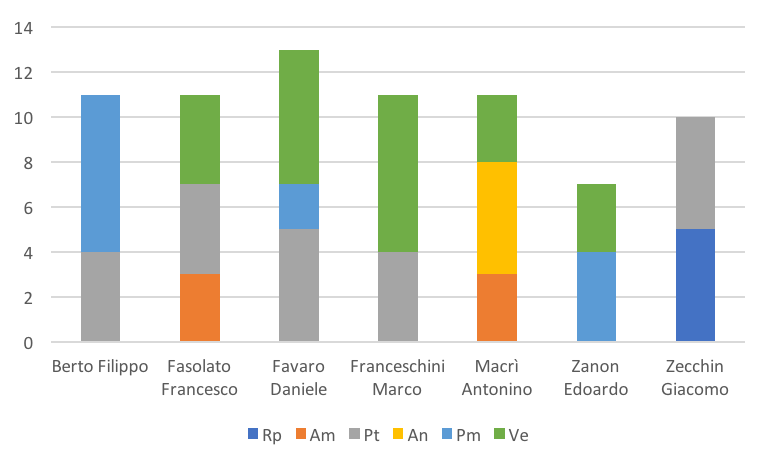
\includegraphics[width=\textwidth]{Preventivo/Immagini/fase6_oreRuoloPersona.png}
				\caption{Sesto Periodo - Riassunto ore di lavoro per persona}
			\end{figure}	

			\newpage
			\paragraph{Prospetto economico}
			Il costo di ogni ruolo è indicato di seguito:
			\begin{table}[h]
				\centering
				\begin{tabular}{l * {2}{c}}
				\toprule
				\textbf{Ruolo} & \textbf{Ore} & \textbf{Costo (\euro{})} \\
				\midrule
				Responsabile & 5 & 150,00 \\
				%\midrule
				Amministratore & 6 & 120,00 \\
				%\midrule
				Progettista & 22 & 484,00 \\
				%\midrule
				Analista & 5 & 125,00 \\		
				%\midrule
				Programmatore & 13 & 195,00 \\		
				%\midrule
				Verificatore & 23 & 345,00 \\				
				\midrule		
				\textbf{Totale} & 74 & 1.419,00 \\
				\bottomrule	
				\end{tabular}
				\caption{Sesto Periodo - Prospetto economico}		
			\end{table}
			
			Riassumendo la precedente tabella con due pie chart:	
			\begin{figure}[!h]
				\centering
				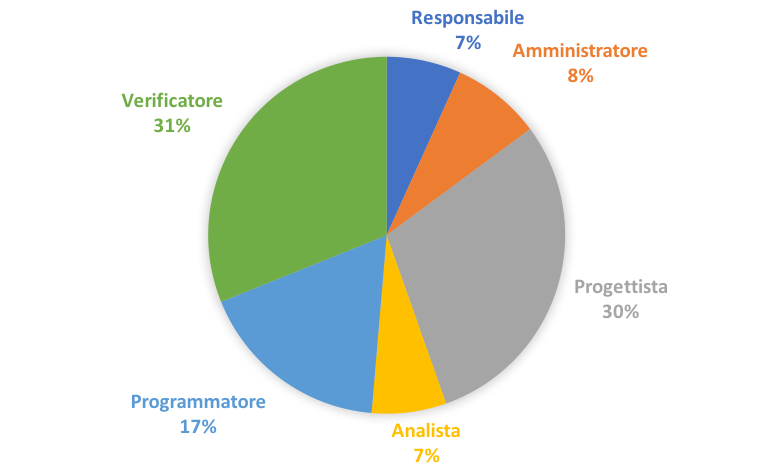
\includegraphics[width=\textwidth]{Preventivo/Immagini/fase6_oreRuolo.png}
				\caption{Sesto Periodo - Riassunto ore di lavoro per ruolo}
			\end{figure}	
			\newpage
			\begin{figure}[!h]
				\centering
				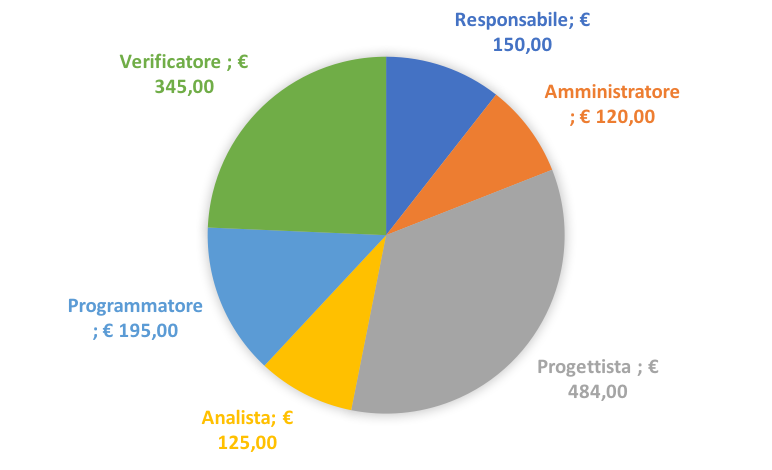
\includegraphics[width=\textwidth]{Preventivo/Immagini/fase6_costoRuolo.png}
				\caption{Sesto Periodo - Riassunto costo per ruolo}
			\end{figure}	

		\newpage
		\subsubsection{Settimo Periodo}
			\paragraph{Suddivisione del lavoro}
			Ogni componente del gruppo \kpanic\ rivestirà i seguenti ruoli:
			\begin{table}[h]
				%\centering
				\begin{tabularx}{\textwidth}{l * {6}{C} c}
				\toprule
				\textbf{Nominativo} & \textbf{Rp} & \textbf{Am} & \textbf{Pt} & \textbf{An} & \textbf{Pm} & \textbf{Ve} & \textbf{Ore totali} \\
				\midrule
				Berto Filippo &	0 & 4 & 0 & 0 & 10 & 0 & 14 \\
				%\midrule
				Fasolato Francesco & 0 & 0 & 0 & 0 & 9 & 5 & 14 \\
				%\midrule
				Favaro Daniele & 0 & 0 & 0 & 0 & 0 & 12 & 12 \\
				%\midrule
				Franceschini Marco & 0 & 0 & 6 & 0 & 0 & 8 & 14 \\
				%\midrule
				Macrì Antonino & 0 & 0 & 6 & 0 & 0 & 8 & 14 \\
				%\midrule
				Zanon Edoardo &	3 & 0 & 0 & 0 & 4 & 8 & 15 \\
				%\midrule
				Zecchin Giacomo & 5 & 0 & 0 & 0 & 0 & 8 & 13 \\
				\midrule
				\textbf{Ore Totali Ruolo} & 8 & 4 & 12 & 0 & 23 & 49 & 96 \\
				\bottomrule
				\end{tabularx}
				\caption{Settimo Periodo - Suddivisione delle ore di lavoro}		
			\end{table}
			
			Riassumendo la precedente tabella con un bar chart:	
			\begin{figure}[!h]
				\centering
				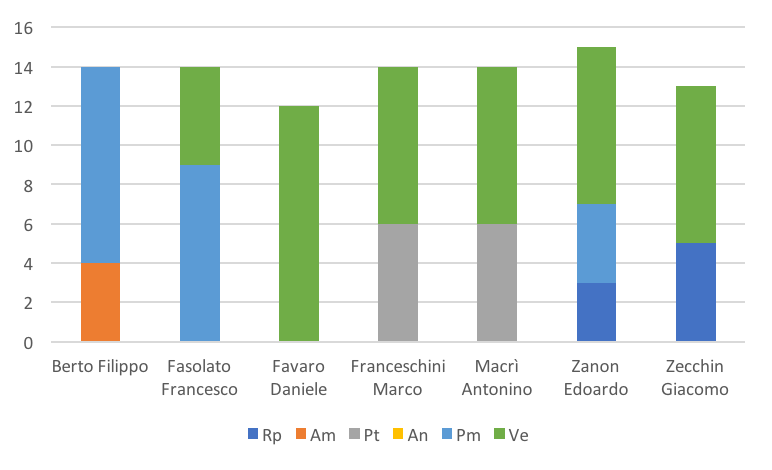
\includegraphics[width=\textwidth]{Preventivo/Immagini/fase7_oreRuoloPersona.png}
				\caption{Settimo Periodo - Riassunto ore di lavoro per persona}
			\end{figure}	

			\newpage
			\paragraph{Prospetto economico}
			Il costo di ogni ruolo è indicato di seguito:
			\begin{table}[h]
				\centering
				\begin{tabular}{l * {2}{c}}
				\toprule
				\textbf{Ruolo} & \textbf{Ore} & \textbf{Costo (\euro{})} \\
				\midrule
				Responsabile & 8 & 240,00 \\
				%\midrule
				Amministratore & 4 & 80,00 \\
				%\midrule
				Progettista & 12 & 264,00 \\
				%\midrule
				Analista & 0 & 0,00 \\		
				%\midrule
				Programmatore & 23 & 345,00 \\		
				%\midrule
				Verificatore & 49 & 735,00 \\				
				\midrule		
				\textbf{Totale} & 96 & 1.664,00 \\
				\bottomrule	
				\end{tabular}
				\caption{Settimo Periodo - Prospetto economico}		
			\end{table}
			
			Riassumendo la precedente tabella con due pie chart:	
			\begin{figure}[!h]
				\centering
				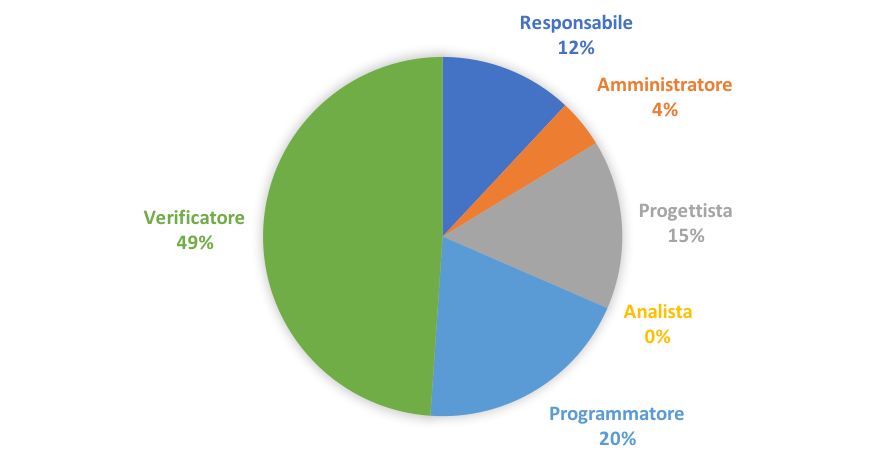
\includegraphics[width=\textwidth]{Preventivo/Immagini/fase7_oreRuolo.png}
				\caption{Settimo Periodo - Riassunto ore di lavoro per ruolo}
			\end{figure}	
			\newpage
			\begin{figure}[!h]
				\centering
				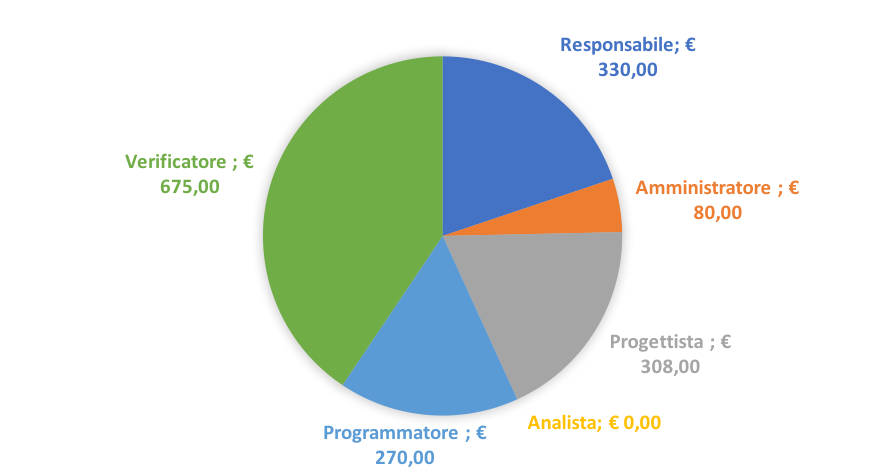
\includegraphics[width=\textwidth]{Preventivo/Immagini/fase7_costoRuolo.png}
				\caption{Settimo Periodo - Riassunto costo per ruolo}
			\end{figure}	

	\newpage
	\subsection{Riepilogo}
		\subsubsection{Ore totali}
			\paragraph{Suddivisione del lavoro}
			Vengono riportate le ore totali che ogni componente del gruppo \kpanic\ dedicherà per ogni ruolo a rotazione:
			\begin{table}[h]
				%\centering
				\begin{tabularx}{\textwidth}{l * {6}{C} c}
				\toprule
				\textbf{Nominativo} & \textbf{Rp} & \textbf{Am} & \textbf{Pt} & \textbf{An} & \textbf{Pm} & \textbf{Ve} & \textbf{Ore totali} \\
				\midrule
				Berto Filippo &	13 & 17 & 22 & 30 & 37 & 16 & 135 \\
				%\midrule
				Fasolato Francesco & 9 & 22 & 26 & 12 & 15 & 51 & 135 \\
				%\midrule
				Favaro Daniele & 14 & 9 & 22 & 18 & 15 & 61 & 139 \\
				%\midrule
				Franceschini Marco & 17 & 12 & 19 & 15 & 30 & 46 & 139 \\
				%\midrule
				Macrì Antonino & 11 & 24 & 15 & 29 & 16 & 45 & 140 \\
				%\midrule
				Zanon Edoardo &	18 & 14 & 27 & 26 & 31 & 23 & 139 \\
				%\midrule
				Zecchin Giacomo & 14 & 19 & 18 & 29 & 21 & 36 & 137 \\
				\midrule			
				\textbf{Ore Totali Ruolo} & 96 & 117 & 149 & 159 & 165 & 278 & 964 \\
				\bottomrule
				\end{tabularx}
				\caption{Suddivisione delle ore totali di lavoro}		
			\end{table}

			Riassumendo la precedente tabella con un bar chart:
			\begin{figure}[!h]
				\centering
				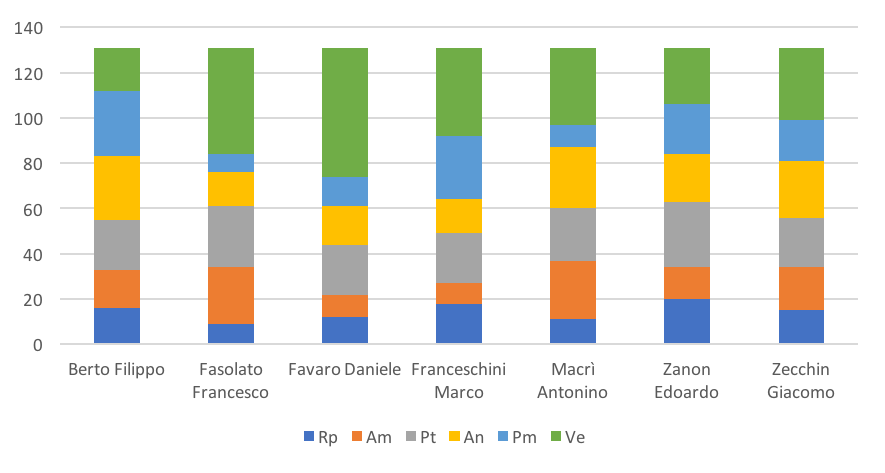
\includegraphics[width=\textwidth]{Preventivo/Immagini/totale_oreRuoloPersona.png}
				\caption{Riassunto ore totali di lavoro per persona}
			\end{figure}	
			
			\newpage
			\paragraph{Prospetto economico}
			Il costo di ogni ruolo è indicato di seguito:
			\begin{table}[h]
				\centering
				\begin{tabular}{l * {2}{c}}
				\toprule
				\textbf{Ruolo} & \textbf{Ore} & \textbf{Costo (\euro{})} \\
				\midrule
				Responsabile & 94 & 2.820,00 \\
				%\midrule
				Amministratore & 114 & 2.280,00 \\
				%\midrule
				Progettista & 149 & 3.278,00 \\
				%\midrule
				Analista & 145 & 3.625,00 \\		
				%\midrule
				Programmatore & 165 & 2.475,00 \\		
				%\midrule
				Verificatore & 269 & 4.035,00 \\				
				\midrule		
				\textbf{Totale} & 936 & 18.513,00 \\
				\bottomrule	
				\end{tabular}
				\caption{Prospetto economico totale}		
			\end{table}
			
			Riassumendo la precedente tabella con due pie chart:	
			\begin{figure}[!h]
				\centering
				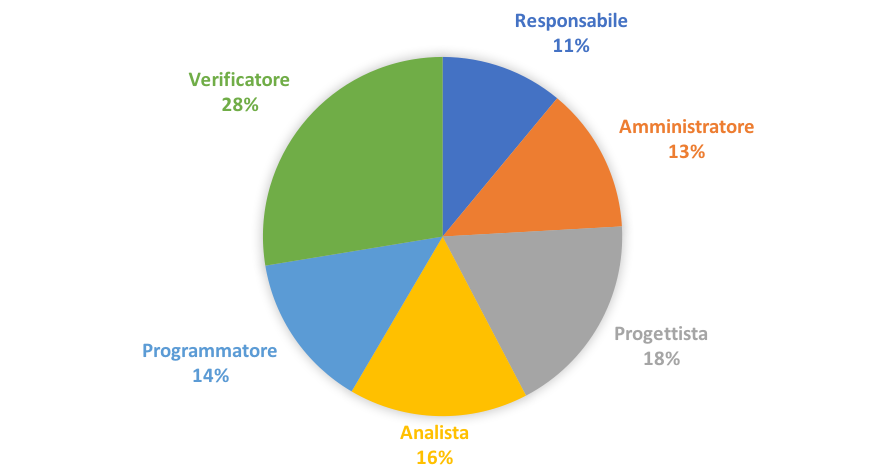
\includegraphics[width=\textwidth]{Preventivo/Immagini/totale_oreRuolo.png}
				\caption{Riassunto ore totali di lavoro per ruolo}
			\end{figure}	
			\newpage
			\begin{figure}[!h]
				\centering
				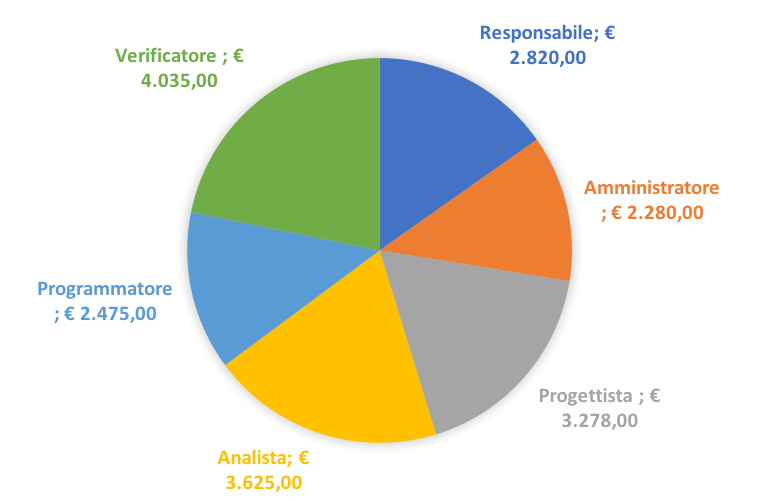
\includegraphics[width=\textwidth]{Preventivo/Immagini/totale_costoRuolo.png}
				\caption{Riassunto costo totale per ruolo}
			\end{figure}	

		\newpage
		\subsubsection{Ore di investimento}
			\paragraph{Suddivisione del lavoro}
			Ogni componente del gruppo \kpanic\ rivestirà i seguenti ruoli:
			\begin{table}[h]
				%\centering
				\begin{tabularx}{\textwidth}{l * {6}{C} c}
				\toprule
				\textbf{Nominativo} & \textbf{Rp} & \textbf{Am} & \textbf{Pt} & \textbf{An} & \textbf{Pm} & \textbf{Ve} & \textbf{Ore totali} \\
				\midrule
				Berto Filippo &	0 & 13 & 0 & 14 & 0 & 4 &  31 \\
				%\midrule
				Fasolato Francesco & 9 & 9 & 0 & 0 & 0 & 14 & 32 \\
				%\midrule
				Favaro Daniele & 14 & 0 & 0 & 13 & 0 & 8 & 35 \\
				%\midrule
				Franceschini Marco & 0 & 12 & 0 & 12 & 0 & 11 & 35 \\
				%\midrule
				Macrì Antonino & 11 & 8 & 0 & 9 & 0 & 8 & 36 \\
				%\midrule
				Zanon Edoardo &	0 & 14 & 0 & 16 & 0 & 5 & 35 \\
				%\midrule
				Zecchin Giacomo & 0 & 11 & 0 & 18 & 0 & 5 & 34 \\
				\midrule			
				\textbf{Ore Totali Ruolo} & 34 & 67 & 0 & 82 & 0 & 55 & 238 \\
				\bottomrule
				\end{tabularx}
				\caption{Suddivisione delle ore investite di lavoro}		
			\end{table}

			Riassumendo la precedente tabella con un bar chart:	
			\begin{figure}[!h]
				\centering
				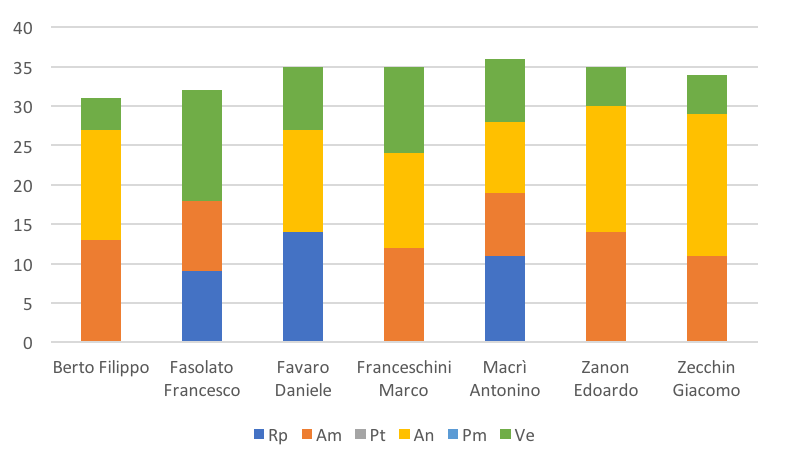
\includegraphics[width=\textwidth]{Preventivo//Immagini/investito_oreRuoloPersona.png}
				\caption{Riassunto ore di lavoro investite per persona}
			\end{figure}	
			
			\newpage
			\paragraph{Prospetto economico}
			Il costo di ogni ruolo è indicato di seguito:
			\begin{table}[h]
				\centering
				\begin{tabular}{l * {2}{c}}
				\toprule
				\textbf{Ruolo} & \textbf{Ore} & \textbf{Costo (\euro{})} \\
				\midrule
				Responsabile & 34 & 1.020,00 \\
				%\midrule
				Amministratore & 67 & 1.340,00 \\
				%\midrule
				Progettista & 0 & 0,00 \\
				%\midrule
				Analista & 82 & 2.050,00 \\		
				%\midrule
				Programmatore & 0 & 0,00 \\		
				%\midrule
				Verificatore & 55 & 825,00 \\				
				\midrule		
				\textbf{Totale} & 238 & 5.235,00 \\
				\bottomrule	
				\end{tabular}
				\caption{Prospetto economico investimento}		
			\end{table}
			
			Riassumendo la precedente tabella con due pie chart:	
			\begin{figure}[!h]
				\centering
				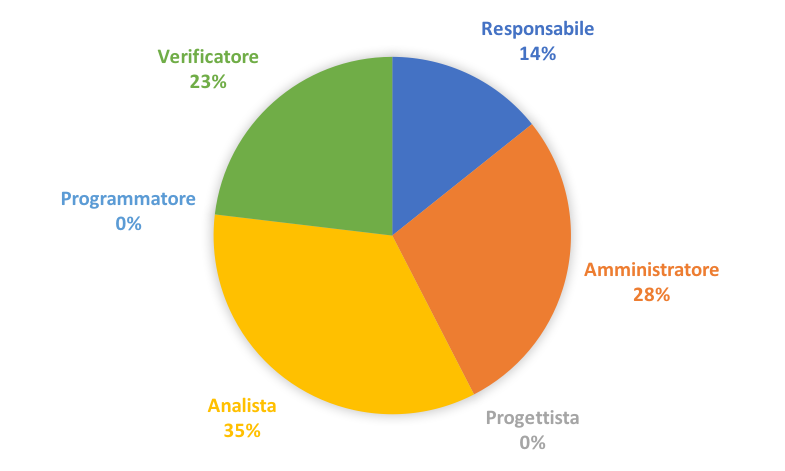
\includegraphics[width=\textwidth]{Preventivo/Immagini/investito_oreRuolo.png}
				\caption{Riassunto ore investite di lavoro per ruolo}
			\end{figure}	
			\newpage
			\begin{figure}[!h]
				\centering
				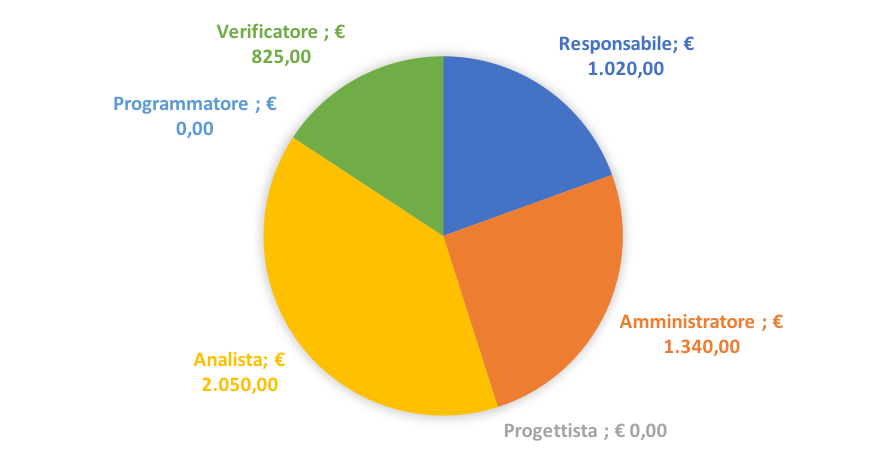
\includegraphics[width=\textwidth]{Preventivo/Immagini/investito_costoRuolo.png}
				\caption{Riassunto costo investimento per ruolo}
			\end{figure}
	
		\newpage
		\subsubsection{Ore rendicontate}
			\paragraph{Suddivisione del lavoro}
			Vengono riportate le ore totali che ogni componente del gruppo \kpanic\ dedicherà per ogni ruolo a rotazione:
			\begin{table}[h]
				%\centering
				\begin{tabularx}{\textwidth}{l * {6}{C} c}
				\toprule
				\textbf{Nominativo} & \textbf{Rp} & \textbf{Am} & \textbf{Pt} & \textbf{An} & \textbf{Pm} & \textbf{Ve} & \textbf{Ore totali} \\
				\midrule
				Berto Filippo &	13 & 4 & 22 & 16 & 37 & 12 & 104 \\
				%\midrule
				Fasolato Francesco & 0 & 13 & 26 & 10 & 15 & 37 & 103 \\
				%\midrule
				Favaro Daniele & 0 & 9 & 22 & 5 & 15 & 53 & 104 \\
				%\midrule
				Franceschini Marco & 17 & 0 & 19 & 3 & 30 & 35 & 104 \\
				%\midrule
				Macrì Antonino & 0 & 16 & 15 & 20 & 16 & 37 & 104 \\
				%\midrule
				Zanon Edoardo &	18 & 0 & 27 & 10 & 31 & 18 & 104 \\
				%\midrule
				Zecchin Giacomo & 14 & 8 & 18 & 11 & 21 & 31 & 103 \\
				\midrule			
				\textbf{Ore Totali Ruolo} & 62 & 50 & 149 & 77 & 165 & 223 & 726 \\
				\bottomrule
				\end{tabularx}
				\caption{Suddivisione delle ore totali di lavoro}		
			\end{table}

			Riassumendo la precedente tabella con un bar chart:
			\begin{figure}[!h]
				\centering
				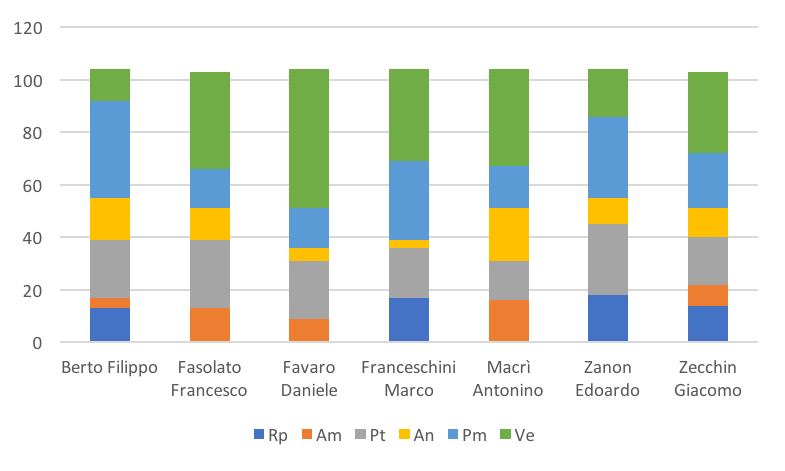
\includegraphics[width=\textwidth]{Preventivo/Immagini/rendicontato_oreRuoloPersona.png}
				\caption{Riassunto ore totali di lavoro per persona}
			\end{figure}	
			
			\newpage
			\paragraph{Prospetto economico}
			Il costo di ogni ruolo è indicato di seguito:
			\begin{table}[h]
				\centering
				\begin{tabular}{l * {2}{c}}
				\toprule
				\textbf{Ruolo} & \textbf{Ore} & \textbf{Costo (\euro{})} \\
				\midrule
				Responsabile & 62 & 1.860,00 \\
				%\midrule
				Amministratore & 50 & 1.000,00 \\
				%\midrule
				Progettista & 149 & 3.278,00 \\
				%\midrule
				Analista & 77 & 1.925,00 \\		
				%\midrule
				Programmatore & 164 & 2.465,00 \\		
				%\midrule
				Verificatore & 223 & 3.145,00 \\				
				\midrule		
				\textbf{Totale} & 726 & 13.883,00 \\
				\bottomrule	
				\end{tabular}
				\caption{Prospetto economico totale}		
			\end{table}
			
			Riassumendo la precedente tabella con due pie chart:	
			\begin{figure}[!h]
				\centering
				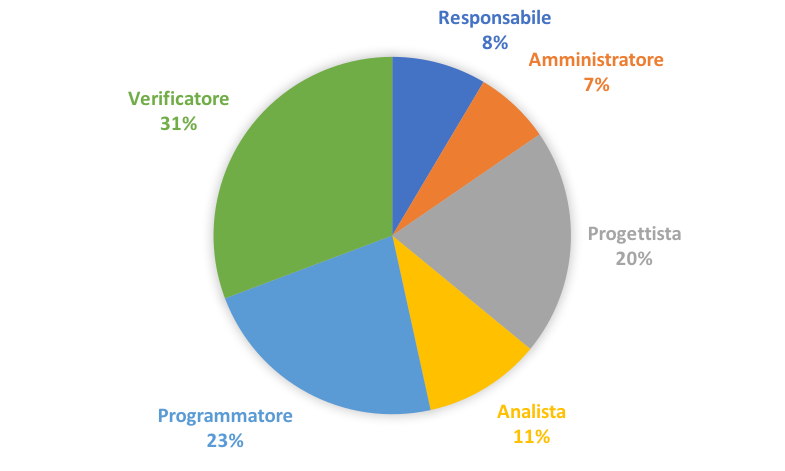
\includegraphics[width=\textwidth]{Preventivo/Immagini/rendicontato_oreRuolo.png}
				\caption{Riassunto ore totali di lavoro per ruolo}
			\end{figure}	
			\newpage
			\begin{figure}[!h]
				\centering
				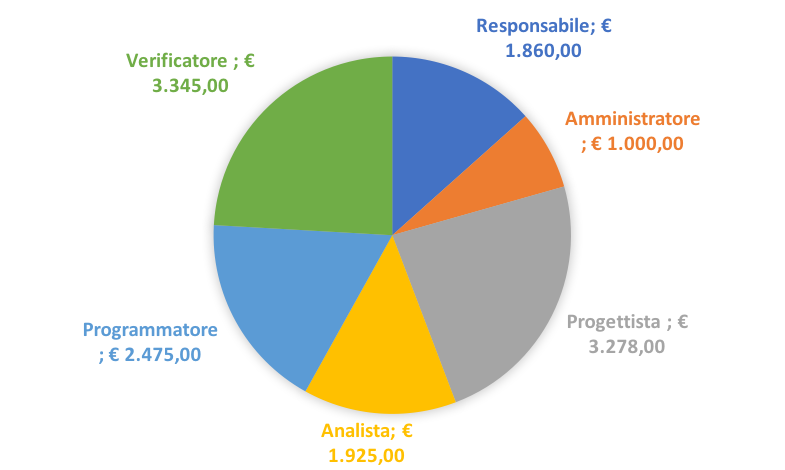
\includegraphics[width=\textwidth]{Preventivo/Immagini/rendicontato_costoRuolo.png}
				\caption{Riassunto costo totale per ruolo}
			\end{figure}
			
			\paragraph{Resoconto economico} Dopo la Revisione dei Requisiti sono state apportate le dovute correzioni alle tabelle del preventivo viste le ore aggiuntive che sono state necessarie per affrontare la prima consegna. Questa modifica ha portato ad una variazione del costo preventivato con una riduzione a finire di 6\euro.

\end{document}